% 1.2.WhenUsedCMake.tex
%	Last update: 2019/10/03 F.Kanehori
%\newpage
\subsection{CzE2SHJQPHzlgjQB}
\label{subsec:WhenUsedCMake}

\noindent
CMake\KLUDGE は、\VS \KLUDGE やmake\KLUDGE のように
\KLUDGE ソースコードのビルドやデバッグの制御をすることを目的としたツールではなく、
\KLUDGE ビルドの自動化を図るためのツールです。
CMake\KLUDGE は、\CMakeLists{}\KLUDGE というパラメータファイルから
solution/project file (Windows \VS)\KLUDGE やMakefile (unix make)\KLUDGE を自動的に生成します
(unix\KLUDGE のconfigure\KLUDGE に近いものと考えていただいてよいでしょう)\KLUDGE 。

\medskip
\noindent
Cmake\KLUDGE はout of source (out of place)\KLUDGE によるビルドに対応しています。
\KLUDGE これはソースツリーの「外側」にビルドツリーを生成する機能で、次のような特徴があります。
\Vskip{-.5\baselineskip}
\begin{itemize}
  \item	\KLUDGE 互いに干渉しない複数のビルドツリーを作成することができる。
  \item	\KLUDGE ビルドツリーが削除されてもソースツリーに影響が及ばない。
\end{itemize}
\Vskip{-.5\baselineskip}
\KLUDGE 我々はCMake\KLUDGE をout of source\KLUDGE の方法で使用します。

\medskip
\noindent
\KLUDGE ソースツリーおよびビルドツリーは次のようになるでしょう
(\KLUDGE 図\ref{fig:SpringheadLibraryTree}\KLUDGE および図\ref{fig:ApplicationTree})\KLUDGE 。

\ifLwarp
\Vskip{-.5\baselineskip}
\begin{narrow}
    \begin{figure}[h]
	\begin{center}
	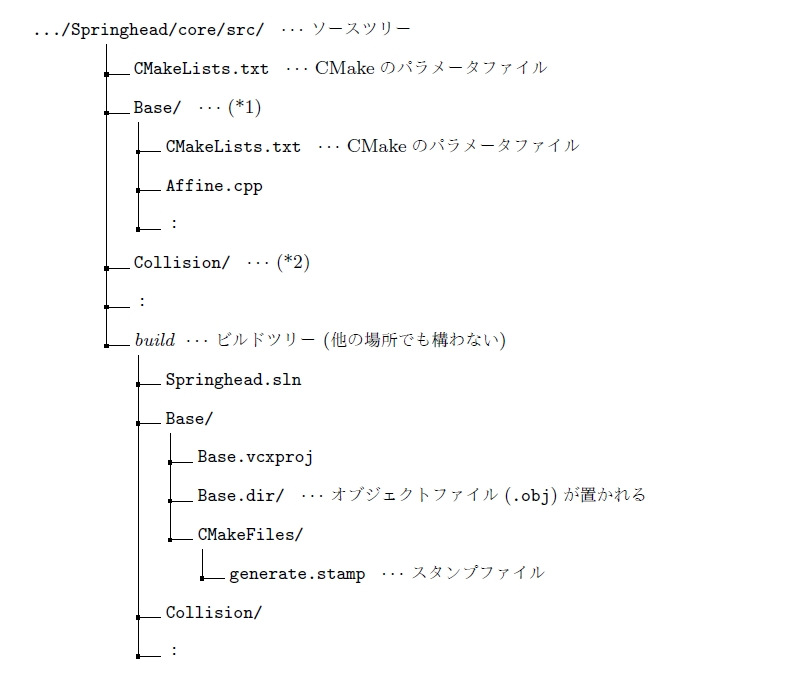
\includegraphics[width=.9\textwidth]{fig/LibraryTree.eps}
	\end{center}
	\caption{Springhead Library\KLUDGE 構成}
	\label{fig:SpringheadLibraryTree}
    \end{figure}
\end{narrow}
\else
\begin{narrow}\begin{figure}[h]
    \begin{narrow}[40pt]\begin{minipage}{\textwidth}
	{\footnotesize{\dirtree{%
		.1 \hspace{-10mm}.../Springhead/core/src/ \Anno{\KLUDGE ソースツリー}.
		.2 CMakeLists.txt \Anno{CMake\KLUDGE のパラメータファイル}.
		.2 Base/ \Anno{(*1)}.
		.3 CMakeLists.txt \Anno{CMake\KLUDGE のパラメータファイル}.
		.3 Affine.cpp.
		.3 \KLUDGE :.
		.2 Collision/ \Anno{(*2)}.
		.2 \KLUDGE :.
		.2 \build \Anno{\KLUDGE ビルドツリー (\KLUDGE 他の場所でも構わない)}.
		.3 Springhead.sln.
		.3 Base/.
		.4 Base.vcxproj.
		.4 Base.dir/ \Anno{\KLUDGE オブジェクトファイル(\tt{.obj})\KLUDGE が置かれる}.
		.4 CMakeFiles/.
		.5 generate.stamp \Anno{\KLUDGE スタンプファイル}.
		.3 Collision/.
		.3 \KLUDGE :.
	}}}
	\medskip
    \end{minipage}\end{narrow}
    \caption{Springhead Library\KLUDGE 構成}
    \label{fig:SpringheadLibraryTree}
\end{figure}\end{narrow}
\fi

\ifLwarp
\Vskip{-.5\baselineskip}
\begin{narrow}
    \begin{figure}[h]
	\begin{center}
	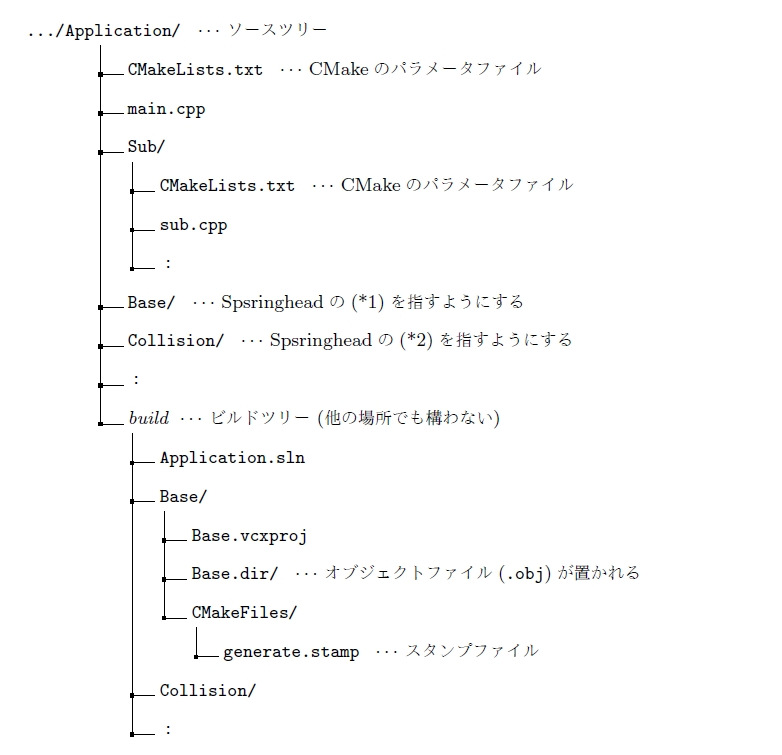
\includegraphics[width=.9\textwidth]{fig/ApplicationTree.eps}
	\end{center}
	\caption{Application\KLUDGE 構成}
	\label{fig:ApplicationTree}
    \end{figure}
\end{narrow}
\Vskip{-1.0\baselineskip}
\else
\begin{narrow}\begin{figure}[h]
    \begin{narrow}[40pt]\begin{minipage}{\textwidth}
	{\footnotesize{\dirtree{%
		.1 \hspace{-10mm}.../Application/ \Anno{\KLUDGE ソースツリー}.
		.2 CMakeLists.txt \Anno{CMake\KLUDGE のパラメータファイル}.
		.2 main.cpp.
		.2 Sub/.
		.3 CMakeLists.txt \Anno{CMake\KLUDGE のパラメータファイル}.
		.3 sub.cpp.
		.3 \KLUDGE :.
		.2 Base/ \Anno{Spsringhead\KLUDGE の(*1)\KLUDGE を指すようにする}.
		.2 Collision/ \Anno{Spsringhead\KLUDGE の(*2)\KLUDGE を指すようにする}.
		.2 \KLUDGE :.
		.2 \build \Anno{\KLUDGE ビルドツリー (\KLUDGE 他の場所でも構わない)}.
		.3 Application.sln.
		.3 Base/.
		.4 Base.vcxproj.
		.4 Base.dir/ \Anno{\KLUDGE オブジェクトファイル(\tt{.obj})\KLUDGE が置かれる}.
		.4 CMakeFiles/.
		.5 generate.stamp \Anno{\KLUDGE スタンプファイル}.
		.3 Collision/.
		.3 \KLUDGE :.
	}}}
	\medskip
    \end{minipage}\end{narrow}
    \caption{Application\KLUDGE 構成}
    \label{fig:ApplicationTree}
\end{figure}\end{narrow}
\fi

\medskip
\noindent
\CMakeLists{}\KLUDGE はメインディレクトリおよびサブディレクトリのそれぞれに作成します。

% end: 1.2.WhenUsedCMake.tex
